\documentclass[11.5pt]{sig-alternate}
\usepackage[defaultlines=3,all]{nowidow}
\usepackage{hyperref}
\usepackage{tabularx}
\usepackage{graphicx}
\usepackage{blindtext}
\usepackage[utf8]{inputenc}
\usepackage[english]{babel}
\usepackage{lastpage}
\usepackage{comment}
\usepackage{dirtytalk}
\usepackage{xcolor}
\usepackage{hanging}
\usepackage{wrapfig}
\usepackage[backend=biber, style=apa]{biblatex}
\addbibresource{notation.bib}
\usepackage{authblk}
\usepackage{caption}
\usepackage{graphicx,subfigure}
\usepackage{authblk}
\usepackage{enumitem}
\usepackage[utf8]{inputenc}
\usepackage{cuted}
\usepackage{fancyhdr}
\pagestyle{fancy}
\usepackage{lipsum}
\renewcommand{\headrulewidth}{0pt}
\renewcommand{\footrulewidth}{0pt}
\setlength\headheight{80.0pt}
\addtolength{\textheight}{-80.0pt}
\chead{%
  \ifcase\value{page}
  % empty test for page = 0
 \or 
\includegraphics[width=\textwidth]{headerImage.png}% page= 1
  \or 
\includegraphics[width=\textwidth]{headerImage.png}% page = 2
  \or 
\includegraphics[width=\textwidth]{headerImage.png}% page = 3
  \or 
\includegraphics[width=\textwidth]{headerImage.png}% page = 4
  \or 
\includegraphics[width=\textwidth]{headerImage.png}% page = 5
  \else
  
\includegraphics[width=\textwidth]{headerImage.png}
  \fi
}

%\chead{
\includegraphics[width=\textwidth]{headerImage.png}}
\fancyfoot[LE,LO]{The SCI – DOT:
A new dimension of scientific innovation for persons with BLV\\           
DOI: 10.14448/jsesd.15.0006}
\fancyfoot[CE,CO]{{ }}
\fancyfoot[RE,RO]{\thepage}
\pagenumbering{arabic}
\hypersetup{
    colorlinks=true,
    urlcolor=blue
}
 
\let\oldabstract\abstract
\let\oldendabstract\endabstract
\makeatletter
\renewenvironment{abstract}
{\renewenvironment{quotation}%
               {\list{}{\addtolength{\leftmargin}{1em} % change this value to add or remove length to the the default
                        \listparindent 1.5em%
                        \itemindent    \listparindent%
                        \rightmargin   \leftmargin%
                        \parsep        \z@ \@plus\p@}%
                \item\relax}%
               {\endlist}%
\oldabstract}
{\oldendabstract}
\makeatother

% Left align captions
\captionsetup{justification   = raggedright,
              singlelinecheck = false}


\begin{document}

\title{The SCI – DOT: \\
A new dimension of scientific innovation for persons with BLV}

\author[1]{\large \color{blue} Ashley N. Nashleanas}



\affil[1]{Independence Science, Inc}
\toappear{}

\maketitle
\begin{@twocolumnfalse} 
\begin{abstract}
\item 
\begin{large}
 \textit{Throughout history, students with blindness and low vision (BLV) have been vastly underrepresented in science, technology, engineering, and mathematics (STEM) disciplines with regards to both K-12 education and post-secondary endeavors (Burgstahler, 1994; Supalo, 2010). This underrepresentation of students with BLV in STEM is due to limitations in technology that allow them to access data in a laboratory setting, thus inhibiting their abilities to partake actively in data acquisition with their peers. The Sci-Dot, a multiline, refreshable braille and tactile graphics display capable of logging scientific data in real time with the support of Vernier Science Education’s (VSE) Go-Direct Bluetooth sensors, stands as a unique innovation for persons with BLV given its capabilities to output multiline, tactile data in real time. The Sci-Dot allows individuals with BLV to collect and analyze data by supplying them with tactile data at their fingertips. Nashleanas reports findings from a usability study to ascertain the technical feasibility of the device – its capability to produce interpretable tactile data in real time. Participants provided feedback that proved the Sci-Dot was technically feasible as a scientific data logger, and more. The Sci-Dot also has the potential to provide a wealth of independence and inclusivity for educational and social activities beyond the laboratory.}\\
 

   
     
     Keywords: SCI-DOT, BLV, Science, Data, Innovation 
 \end{large}     
\end{abstract}
\end{@twocolumnfalse}

%% ABSTRACT


%% AUTHOR INFORMATION

\textbf{*Corresponding Author, Ashley N. Nashleanas}\\
\href{mailto:anashleanas@independencescience.com}{(anashleanas@independencescience.com)} \\
\textit{Submitted Mon Jan 09, 2023 }\\
\textit{Accepted Fri Mar 31 2023} \\
\textit{Published online August 15, 2023} \\
\textit{DOI: 10.14448/jsesd.15.0006} \\

\pagebreak
\pagebreak

\vspace{5mm}
\section*{\vspace{140mm}}
\section*{Introduction}
\begin{large}
Imagine that you are enrolled in a laboratory course and can participate with all senses except for vision. How would you imagine yourself performing laboratory experiments along with your peers? Aside from relying on your peers to do the physical work of pouring, mixing, and weighing, for safety’s sake, you also would be at the mercy of your partners to articulate observations of what occurs as the experiment proceeds. As you can imagine, this experience would relegate you as a student enrolled in a course where the laboratory component is required and integral to the course itself, to the role of passive observer. This high reliance on others to provide you with relevant information would result in many negative emotions such as embarrassment that you have to rely on others to perform activities you would like to perform on your own, as well as a lack of confidence to gain a fundamental understanding of the experiment’s original purpose and significance to advancing your scientific knowledge.

This is what so many students with blindness and low vision, or BLV, encounter when in laboratory settings. Students with BLV historically have found themselves in positions of passivity when enrolled in their laboratory courses, causing them to choose degrees and career paths alternative to science, technology, engineering, and mathematics, or STEM (Burstahler, 1994; Supalo, 2010). However, advancements in STEM access technology have enabled students with BLV to have more equitable experiences in their laboratory courses, allowing them opportunities to operate more as active participants than they have in the past. One of these successful efforts to bring greater equity to the STEM field for students with BLV was the Sci-Voice Talking Lab Quest developed by a collaboration between Vernier Science Education (VSE), a premier science education technology company providing a plethora of tools and materials to students and teachers alike, and staff employed with Independence Science, LLC, a small business whose mission is to empower hands-on \\STEM learning for BLV both individually and as part of a group effort.

The Talking LabQuest adds text-to-speech and other accessibility features to the LabQuest to provide data as audio output to users as they collect and analyze it Utilizing the Talking \\LabQuest, along with data output in tactile graphical form, was a springboard for students with BLV to respond more positively about enrolling in laboratory courses with a greater level of independence in observing data through complementary senses of touching braille-embossed data and hearing, along with confidence that they could use what they accessed to understand lab exercises more on level with their sighted peers.

Although the combination of the Sci-Voice Talking LabQuest and raised line images produced by braille embossers provided students who are BLV with more improved laboratory settings than they had previously, the component of real-time tactile access to data acquired as part of a laboratory experiment was still absent, \\demonstrating that a large gap needed to be filled in the way of STEM access for students with BLV interested in pursuing STEM degrees and employment. When considering all nonvisual senses and how they compare to vision for spatial learning, touch happens to be the closest sense to vision for absorbing spatial information due to the configuration information that touch and movement provide about an environment that sound alone cannot (Millar, 1994; Nashleanas, 2018; Zebehazy \& Wilton, 2014a;2014b;\\2014c;). In addition, the works of these researchers demonstrate that receiving information in real time along with their sighted peers is key to allowing students with BLV to contribute more interactively in high-level thinking skills, as opposed to receipt of that information after the fact, as happens commonly for persons with BLV in STEM spaces.

In order to make yet a greater advancement in STEM access technology for students with BLV to partake more equitably in laboratory components of their science courses in a way they have never been able to do previously, an opportunity to construct a device capable of multiline, tactile, and real-time scientific data acquisition came through the National Science Foundation Small Business Innovation Research (NSF/SBIR) program in the form of a funded grant proposal (Nashleanas, 2022). For the Phase I effort of this grant, Nashleanas and Williams spearheaded the development of the Sci-Dot, a multiline, refreshable braille and tactile graphics tablet intended for real-time data acquisition using the VSE suite of Go-Direct Bluetooth sensors to feed data to the tablet. The Sci-Dot is multi-configurational, with options of use with 1, 2, or 4 modules. On each module is a total of 48 braille cells, spanning twelve cells in the horizontal direction and four cells in the vertical direction. Nashleanas provides visual depictions, and written descriptions of those depictions, as a way to help readers visualize the concept of the Sci-Dot.

Figure 1 shows the Sci-Dot as represented by a single module. A single module resembles one half of a refreshable braille display, where the user can choose to type with either the left or right hand depending on the orientation of the typing keys.

\pagebreak
\begin{figure}[htp]
    \centering
    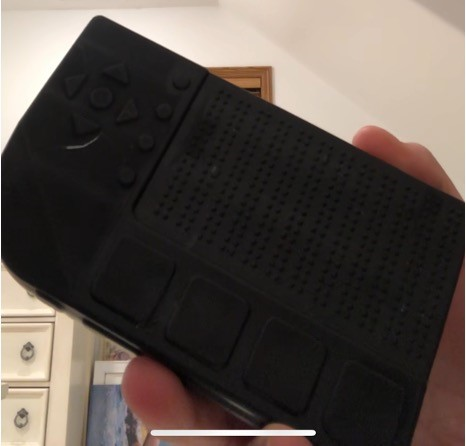
\includegraphics[width=8cm]{figure 1.png}
 \caption{the Sci-Dot as represented by a single module }
    \label{the Sci-Dot as represented by a single module}
\end{figure}

Figure 2 shows the Sci-Dot as represented by a pair of two modules held together. Here, users are able to type with both hands as they would using a refreshable braille display, and the cells above the keys provide four lines of refreshable braille.

\begin{figure}[htp]
    \centering
    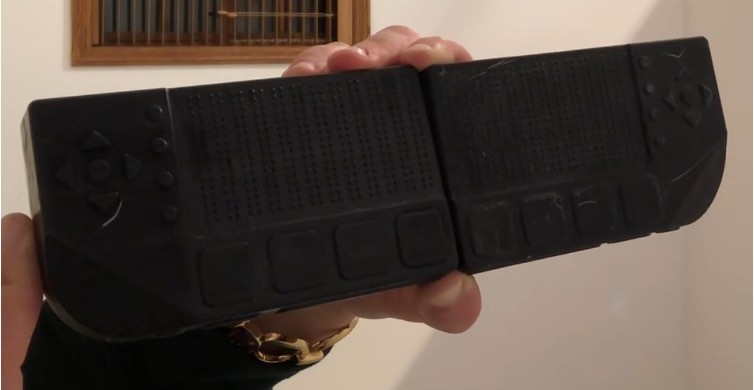
\includegraphics[width=8cm]{figure 2.png}
 \caption{the Sci-Dot as represented by a pair of two modules held together }
    \label{the Sci-Dot as represented by a pair of two modules held together}
\end{figure}

Figure 3 shows the Sci-Dot in quadrant form. In this representation of the Sci-Dot, the four modules are in a square configuration, with the braille cells facing into each other with all keys on the edges of the square. 

   \begin{figure}[htp]
    \centering
    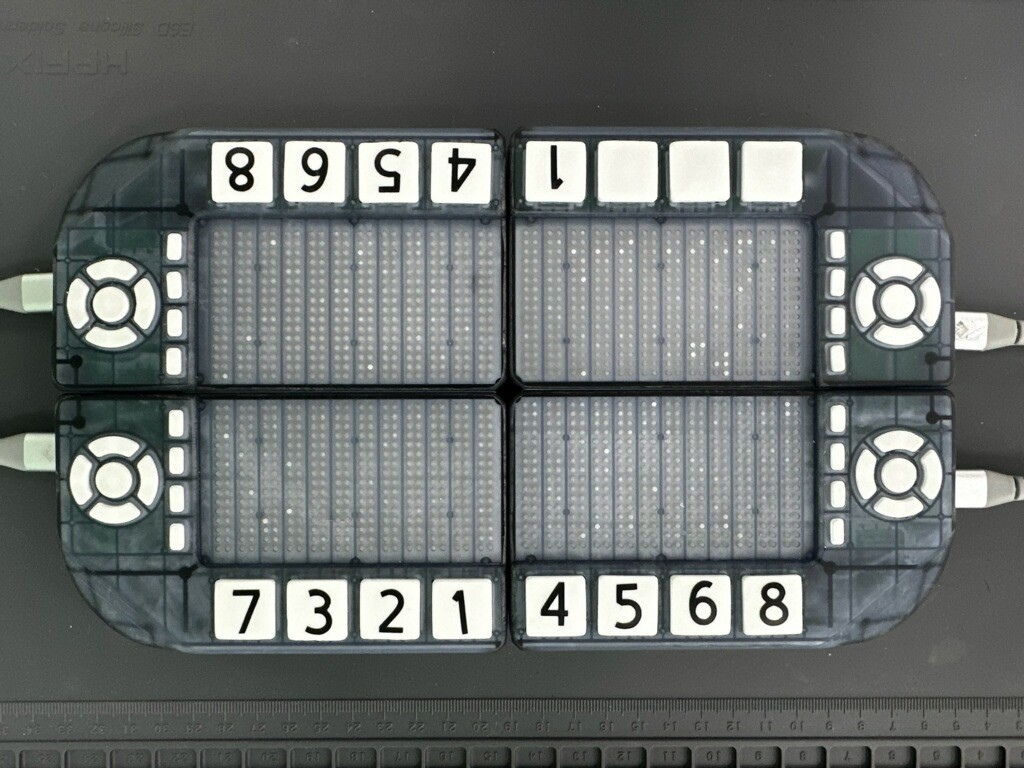
\includegraphics[width=8cm]{figure 3.png}
 \caption{the Sci-Dot in quadrant form }
    \label{the Sci-Dot in quadrant form}
\end{figure}

The mere novelty of the Sci-Dot meant that technical feasibility testing needed to take place to determine whether the Sci-Dot was capable of scientific data acquisition upon connection to VSE’s sensors, and if so, the quality of output it would produce. 

As such, the research questions to be addressed as part of the Phase I effort were: 
\begin{enumerate}
    \item Will the authors be able to leverage the VSE GoDirect Bluetooth sensors to do quantifiable real-time data collection and analysis in a dynamic tactile graphics refreshable braille display supported by text to speech?
    \item How do persons with BLV perceive the level of interpretability of real-time tactile graphics when using the Sci-Dot? 
\end{enumerate}
These research questions laid the blueprint for forming and testing the hypothesis that it would be technically feasible for the Sci-Dot to perform scientific data collection in real time science laboratory settings. Nashleanas relied on Mertens’ disability theory (2003, as cited in \\Creswell, 2007) as the lens for conducting this study. Nashleanas and their collaborators are affiliated with a small business composed entirely of individuals with BLV who have earned advanced degrees in a variety of STEM disciplines. Disability theory is suitable for explaining the relevance of the research conducted Nashleanas and their collaborators as part of this small business. Disability theory demonstrates that the term ‘disability’ not as a defect, but rather as a unique set of differences that allows for individuals with disabilities opportunities to apply their skill sets in ways that create positive communal perceptions of disability. Demonstrating technical success with the Sci-Dot would prove disability theory applicable to this small business as the lead developer, along with individuals willing to participate in testing as the user base. The details of this effort are described in the following sections.
\section*{Data collection}
The purpose of the data collection session was to receive user feedback on the usability of the Sci-Dot prototype, specifically its capability as a multiline, refreshable, real-time scientific data logger. The nature and newness of the Sci-Dot was reason for selecting a data collection setting that holds many individuals with BLV who have varying levels of braille and tactile graphics literacy. 

The researchers therefore decided to conduct data collection sessions through the National Federation of the Blind, a consumer organization known for hosting large numbers of persons with BLV. Nashleanas and her collaborators conducted a qualitative study with ten participants. The researchers held a total of four sessions, each lasting 90 minutes in length.

They received institutional review board (IRB) approval for all data collection and analysis procedures. 

\section*{Data collection procedure}

All data collection sessions were recorded and transcribed on a password-protected computer. Pseudonyms were used to preserve participant identities for data analysis purposes. All consent forms were kept in a locked space. We familiarized participants with the Sci-Dot through an introductory chemistry experiment that involved holding and releasing a temperature probe as participants noted changes in temperature over time. Following this exercise, the researchers elicited information from participants with three Likert-scale questions provided a scale of 5 to 1, five being strongly agree, indicating positive aspects of the Sci-Dot, and 1 being strongly disagree indicating features in need of improvement. The Likert-scale questions were: “The tactile graphics were easy to understand”, “The Sci-Dot made it possible for me to perform the science activity independently.” And “If I were to take a science lab course in the future, I would like to use the Sci-Dot in the course.” We then asked open-ended questions for participant feedback on the capability of the Sci-Dot to act as a scientific data logger.

\section*{Recruitment}
Nashleanas used theoretical sampling (Creswell, 2007) to recruit participants by distributing an invitation email for conference attendees to participate. Upon expressing interest, Nashleanas used a screening process to determine whether or not those interested were fit for the study. Each participant was at least 18 years of age, literate in braille and tactile graphics, and took at least one science course throughout their lives. All participants resided in the United States. The sample was ethnically diverse (40\% Caucasian and 60\% other racial backgrounds). Four males and six females participated, with ten states represented. 

Table 1 provides readers with more specifics of these participant demographics.

\section*{\textit{ Table 1. Participant demographics}}

\begin{tabular}{ | m{3em} | m{3cm}| m{3cm}|}
 \hline
Gender & State of \newline residence & Level of \newline Blindness \\ 
 \hline
 male & New York & totally blind \\ 
 \hline
 male & Michigan & legally blind \\ 
 \hline
 female & New Jersey & totally blind \\ 
 \hline
 male & Nevada & legally blind \\ 
 \hline
female & Nebraska & legally blind \\ 
 \hline
female & Maryland & legally blind \\ 
 \hline
 male & Texas & legally blind \\ 
 \hline
 female & Arizona & legally blind \\ 
 \hline
 female & Georgia & legally blind \\ 
 \hline
female & Iowa & legally blind \\ 
\hline
\end{tabular}\\

\section*{Data Analysis}

Nashleanas used the grounded theory methodology (Creswell, 2007) to analyze the data for this qualitative study. Grounded theory, the approach researchers commonly choose upon \\forming hypotheses for testing, is the most scientific form of qualitative methodologies. It is a stepwise process Creswell further explains as allowing the researcher to “move beyond description and to generate or discover a theory, an abstract analytical schema of a process” (p. 62). She chose grounded theory because they anticipated participants would provide feedback on the Sci-Dot’s ability to do data acquisition as well as how it could be a prominent tool for enhancing social and educational inclusivity. 

Each researcher utilized their own forms of open coding by gleaning the data corpus to identify participant feedback relevant to functionality and usability of the device, such as comments about the shape and live refreshing of the braille and tactile graphics output by the Sci-Dot. The coding scheme was refined by using axial coding to group the open codes into categories, then further refined into overarching themes such as independence, quality of data output, portability, and inclusivity beyond scientific data collection. 

Nine out of ten participants reported on the Likert scale that they would be able to collect and analyze data independently using the Sci-Dot.  To the feedback on independence, nine of ten participants responded in agreement to the Likert scale prompt on quality of braille and tactile graphics output. When provided the opportunity to verbalize further, being able to easily identify the shape of the graph instantaneously through tactile means provided participants with the information they needed to explain overall trends when needed. Also, having both the braille and graphical output allowed participants to make comparisons between data in numerical and graphical form. 

One participant was unique from the rest, stating that she did not know whether she would be able to collect and analyze data independently using the Sci-Dot. She claimed her response of “Don’t know” was the result of a lack of recent exposure to tactile graphics. She emphasized that the addition of audio cues would be much to her benefit in understanding her location within a tactile graphical representation. 

Participants provided feedback beyond scientific data acquisition. For example, they spoke fondly of the portability of the device. They appreciated that they could use either the two- or four-module version of the device for data manipulation using the typing keys and exploration on the display. Along with modularity options, participants also appreciated the portability it offered given the ease of transportation from one space to another. 

Participants explicated on the potential for the Sci-Dot to act as a tool for activities such as graph construction, gaming, and note taking. They expressed their excitement regarding the myriad of possibilities the Sci-Dot provided them with for taking ownership of their social and educational well-being in a way that no other device has allowed them to do. The innovation of multiline refreshable braille and tactile graphics stood as participants’ reasoning for believing the Sci-Dot could enhance their social and educational well-being. 

As part of the data analysis process, Nashleanas and Williams utilized the external evaluation services of HigherEdInsight to act as a checkpoint for validation of the data in support of the hypothesis that technical feasibility with the Sci-Dot was possible. Both entities independently coded the data, then convened to exchange their overall understanding of the overarching themes. Nashleanas and HigherEdInsight came to the same conclusions that the Sci-Dot proved successful in real-time scientific data logging using refreshable braille and tactile graphics as well as other educational and social facets.

\section*{Discussion}
As Nashleanas demonstrated in the sections \\above, their efforts were successful in proving that the Sci-Dot is capable of acquiring data when connected to VSE’s suite of sensors, and in addition, providing social and educational inclusivity with common activities that do not involve exercises in a lab. Participants spoke well of the device’s output, deeming it as a versatile educational tool both in and out of the lab. This participant feedback elicits evidence of a successful innovation for Phase I, which has led Nashleanas to pursue a second phase of NSF funding.

\section*{Future Directions}
The innovative success of Phase I provided a motive to identify the next steps for advancing STEM access developments. The Sci-Dot is a device intended for individuals with some level of braille and tactile graphics literacy along with STEM familiarity. In addition, there exist print disabilities other than BLV (e.g., dyslexia (Gonzalez, 2016) and neurodiversity (Haine et al., 2018) that also are underrepresented in STEM disciplines. Nashleanas and her collaborators therefore seek to develop a progressive Web application using VSE’s graphical analysis software, for individuals with print-reading disabilities to utilize tools they have at their avail to perform scientific data collection in a 508-compliant way. With this new effort, Independence Science researchers seek to create a system that will drive improvements to existing access tools and motivate the production of newer access tools. This approach will allow for greater inclusivity among print-reading disabilities for data acquisition, introducing a new take on universal design for STEM.
\section*{Conclusion}
The persistent problem of underrepresentation of persons with BLV studying and employed in STEM provided Nashleanas and her collaborators with the drive to capitalize on their strength as a STEM accessibility leader in a game-changing way. This effort involved shifting the paradigm from data collection and analysis via text-to-speech technologies, to data acquisition via multiline refreshable braille and tactile graphics in real time. Development of the Sci-Dot was a successful proof of technical feasibility. This successful innovation then spawned work toward what is hoped to provide the game-changing solution for a universally accessible STEM experience for students with multiple types of print disabilities.

\include{} 
\section*{References}\par 

\leftskip 0.25in
\parindent -0.25in 
%%%

Burgstahler, S. (1994). Increasing the representation of people with disabilities in science, engineering, and mathematics. \textit{Information Technology and Disability}, 1(4)\\

Creswell, J. W. (2007).\textit{ Qualitative inquiry and research design: Choosing among five approaches} (2nd ed.). Thousand Oaks, CA: Sage Publications.\\

Gonzalez, F. (2016). For some, active learning can be a nightmare. \textit{ASEE Prism}, 26(4), 52.\\

Hain, A., Zaghi, A. E., \& Taylor, C. L. (2018, June). Board 164: Promoting neurodiversity in engineering through undergraduate research opportunities for students with \\ADHD. In \textit{2018 ASEE Annual Conference \& Exposition}.\\

Millar, S. (1994). \textit{Understanding and representing space: Theory and evidence from studies with blind and sighted children}. Clarendon Press/Oxford University Press.\\

Nashleanas, A.N.  (2018). Graph accessibility and comprehension for the blind: \textit{A challenge of its own kind} (Doctoral dissertation, Iowa State University)\\

Nashleanas, A.N. (2022). Synergizing Braille and Science: Real-time Accessibility of Tactile Graphics in Laboratory Settings for Blind and Low Vision (BLV) Students. (Award \#2112636)\\

National Federation of the Blind (2022). Blindness Statistics. Retrieved Monday, December 19, 2022 from \\<https://nfb.org/resources/blindness-statistics.\\

Supalo, C. A. (2010). \textit{Teaching chemistry and other sciences to blind and low-vision students through hands-on learning experiences in high school science laboratories}. The Pennsylvania State University.\\

Zebehazy, K. T.,\& Wilton, A. P. (2014a). Quality, importance, and instruction: The perspective of teachers of students with visual impairments on student graphic use. \textit{Journal of Visual Impairment} \& Blindness, 108(1), 5–16.\\

Zebehazy, K. T., \& Wilton, A. P. (2014b). Charting success: The experience of teachers of students with visual impairments in promoting graphic use by students.\textit{ Journal of Visual Impairment \& Blindness}, 108(4), 263–274.\\

Zebehazy, K. T., \& Wilton, A. P. (2014c). Straight from the Source: Perceptions of Students with Visual Impairments about Graphic Use. \textit{Journal of Visual Impairment \& Blindness}, 108(4), 275-286.\\

\end{large}
\end{document}
